% Includable product documentation for the main thesis document.
% This file is intended to be included from NeckebroekKyanuBP.tex.
% Do not compile standalone.

\chapter{Uitwerking}
\label{ch:uitwerking}

Dit hoofdstuk bundelt het projectoverzicht, de dataverwerking, de modelimplementatie en de uitvoering van de pipeline.

\section{Projectstructuur}

In de onderstaande figuur wordt de mappenstructuur van het project weergegeven. Ik ga hierin te werk door eerst de centrale configuratie en de pipeline te bespreken, daarna de data-architectuur en ten slotte de code-indeling in preprocessing, modeltraining en evaluatie.

\begin{verbatim}
misinformatie_detectie/
├── config.yaml                   # Centrale configuratie
├── requirements.txt              # Python dependencies
├── run_pipeline.py               # Volledige pipeline
├── setup.py                      # Package-installatie
├── data/
│   ├── raw/                      # Onverwerkte brondata, inclusief LIAR
│   ├── processed/                # Geschoonde train/val/test splits
│   └── mastodon/                 # Verzamelde Mastodon-berichten
├── src/
│   ├── utils.py
│   ├── preprocessing/
│   │   ├── mastodon_collector.py
│   │   ├── liar_preprocessor.py
│   │   └── data_merger.py
│   ├── models/
│   │   ├── train_svm.py
│   │   ├── train_logistic_regression.py
│   │   └── train_bert.py
│   └── evaluation/
│       ├── metrics.py
│       ├── evaluate_all.py
│       └── factor_analysis.py
├── notebooks/
│   ├── 01_eda.ipynb
│   └── 02_analyse_rapport.ipynb
├── results/
│   ├── svm/, lr/, bert/
│   └── figures/
└── tests/
\end{verbatim}

De kern van het project bevindt zich in \texttt{run\_pipeline.py}. Dit script start de volledige workflow: data ophalen, preprocessen, modellen trainen en resultaten evalueren. De configuratie in \texttt{config.yaml} maakt het mogelijk om dezelfde pipeline reproduceerbaar uit te voeren met verschillende model- en datainstellingen. De \texttt{requirements.txt} bevat alle Python-pakketten die noodzakelijk zijn voor de uitvoering.

In \texttt{data/raw/} worden de originele gegevens bewaard, inclusief de LIAR-tekstbestanden en de ruwe Mastodon-berichten. Na preprocessing komen de geschoonde en gebalanceerde datasets in \texttt{data/processed/}. De Mastodon-berichten zijn apart opgeslagen in \texttt{data/mastodon/}, omdat deze data rechtstreeks uit de API komt en daarna handmatig is gelabeld.

De programmeercode is opgesplitst in drie domeinen. In \texttt{src/preprocessing/} bevinden zich de scripts voor data-inwinning, tekstopschoning en het samenvoegen van LIAR met Mastodon. In \texttt{src/models/} staat de implementatie van de trainingspipelines voor Support Vector Machine, Logistic Regression en BERT. In \texttt{src/evaluation/} worden de modelprestaties berekend, vergeleken en geanalyseerd.

\section{Technologieën}

Voor dit project is gekozen voor een Python-gebaseerde stack omdat deze zowel traditioneel machine learning als transformer-gebaseerde NLP naadloos ondersteunt. Python 3.11 vormt de basis, omdat deze versie compatibel is met moderne bibliotheken en onderhoudbaarheid bevordert.

Scikit-learn wordt gebruikt voor de traditionele modellen (SVM en Logistic Regression). Deze bibliotheek is geschikt vanwege zijn heldere API, eenvoudige implementatie en bewezen betrouwbaarheid bij tekstclassificatie. Voor het BERT-model is gekozen voor PyTorch in combinatie met Hugging Face Transformers, omdat die combinatie het mogelijk maakt om een voorgetraind transformer-model effectief te fine-tunen op de specifieke Mastodon- en LIAR-data.

Mastodon.py is de gekozen tool voor de Mastodon API-integratie. Deze bibliotheek sluit goed aan op het federatieve karakter van Mastodon en maakt het eenvoudiger om berichten gecontroleerd en reproduceerbaar te verzamelen. NLTK wordt ingezet voor tekstpreprocessing vanwege zijn volwassen tokenizers, stopwoordlijsten en taalhulpmiddelen, terwijl BeautifulSoup4 helpt bij het verwijderen van HTML-achtige tags en andere tekstvervuiling.

SciPy ondersteunt de statistische evaluatie van de resultaten, bijvoorbeeld bij het vergelijken van modelprestaties en het onderbouwen van conclusies met kwantitatieve metrieken. Matplotlib en Seaborn worden gebruikt om de resultaten visueel weer te geven, zoals performance-curves, confusiematrices en factoranalyses.

% ══════════════════════════════════════════════════════════════════
\section{Data en Preprocessing}
\label{sec:data-preprocessing}
% ══════════════════════════════════════════════════════════════════

De gedetailleerde beschrijving van dataverzameling, LIAR-dataset verwerking,
Mastodon API-integratie, tekstopschoning en preprocessinglogica vindt u in
Hoofdstuk~\ref{ch:methodologie}. In deze sectie beperken we ons tot de
praktische implementatie in code.

\section{Dataverwerking Pipeline}

De volledige preprocessing pipeline wordt orchestreerd via het script
\texttt{run\_pipeline.py}. De stappen zijn:

\begin{enumerate}
    \item LIAR-dataset downloaden en converteren naar binaire labels
    \item Mastodon-berichten verzamelen via API (optioneel). Ik heb de Mastodon-testdata met een Python-script uit de publieke API verzameld.
    \item Beide datasets samenvoegen en shufflen
    \item Train/Val/Test splits aanmaken
\end{enumerate}

Alle dataverwerking vindt plaats in \texttt{src/preprocessing/}.

% ══════════════════════════════════════════════════════════════════
\section{Modellen implementeren}
\label{sec:modellen}
% ══════════════════════════════════════════════════════════════════

Deze sectie beschrijft de praktische implementatie van drie modellen.
Theoretische achtergrondinformatie (TF-IDF-wiskunde, SVM-optimalisatie,
transformer-architectuur) vindt u in Hoofdstuk~\ref{ch:methodologie}.

De keuze voor de drie modellen is bewust gemaakt op basis van de specifieke
Mastodon-usecase. Mastodon-berichten zijn tekstueel vaak kort en informeel,
met bijzondere kenmerken zoals Content Warnings en gedecentraliseerde bronherkenning.
Daarom selecteer ik zowel sterke lineaire baselines als een contextueel
transformer-model:

\begin{itemize}
    \item \textbf{Logistic Regression}: een eenvoudige, interpreteerbare baseline
          die in veel tekstclassificatieproblemen verrassend goed presteert.
    \item \textbf{Support Vector Machine}: een robuust, margin-gebaseerd model dat
          goed omgaat met hoge-dimensionale, sparse TF-IDF features.
    \item \textbf{BERT}: een transformer-gebaseerd model dat de semantische
          context van hele zinnen kan vastleggen en daarmee beter kan omgaan met
          de variatie in Mastodon-berichten.
\end{itemize}

Deze combinatie van modellen sluit aan bij de literatuur uit
Hoofdstuk~\ref{ch:stand-van-zaken}, waar zowel traditionele lineaire
classifiers als transformer-gebaseerde modellen als relevante benchmarks
worden genoemd. Andere mogelijkheden zoals Naive Bayes, Random Forest of
RNN/CNN zijn overwogen, maar minder geschikt voor deze dataset:

\begin{itemize}
    \item \textbf{Naive Bayes}: te simplistisch voor de complexere,
          contextuele taalpatronen die in misinformatie voorkomen.
    \item \textbf{Random Forest / Decision Trees}: slecht schaalbaar naar
          hoge-dimensionale TF-IDF features en minder gangbaar in recente
          NLP-literatuur voor tekstclassificatie.
    \item \textbf{RNN/CNN}: meer complex om te trainen en niet zo goed
          ondersteund als de transformer-gebaseerde benadering voor korte
          tekstsegmenten wanneer pre-trained modellen beschikbaar zijn.
\end{itemize}

\section{Logistic Regression}

\textbf{Bestand}: \texttt{src/models/train\_logistic\_regression.py}

Logistic Regression is gekozen als baseline omdat het een eenvoudige,
lineaire classifier is die goed werkt op sparse tekstrepresentaties. In de
context van Mastodon geeft dit model een referentiepunt voor de vraag of
complexere modellen zoals BERT echt een meerwaarde bieden.

\begin{lstlisting}[language=Python, basicstyle=\ttfamily\scriptsize,
  caption={Logistic Regression training pipeline},
  literate={_}{\_}1]
from sklearn.linear_model import LogisticRegression
from sklearn.pipeline import Pipeline
from sklearn.feature_extraction.text import TfidfVectorizer

pipeline = Pipeline([
    ('tfidf', TfidfVectorizer(
        max_features=50000, ngram_range=(1, 2),
        min_df=2, max_df=0.95, sublinear_tf=True
    )),
    ('lr', LogisticRegression(
        C=1.0, max_iter=1000,
        class_weight='balanced', solver='lbfgs'
    ))
])

pipeline.fit(X_train, y_train)
y_pred = pipeline.predict(X_test)
y_proba = pipeline.predict_proba(X_test)[:, 1]
\end{lstlisting}

In deze pipeline wordt eerst een \texttt{TfidfVectorizer} toegepast. Dit
transformeert tekst naar numerieke vectoren op basis van woordfrequenties,
waarbij veel voorkomende woorden worden gedempt en zeldzame maar kenmerkende
woorden relatief hoger scoren. De parameters zijn gekozen om:

\begin{itemize}
    \item \texttt{max\_features=50000}: genoeg representatiecapaciteit,
          zonder te veel ruis toe te laten.
    \item \texttt{ngram\_range=(1, 2)}: zowel losse woorden als woordcombinaties
          (bijv. "mijn de") worden meegenomen.
    \item \texttt{min\_df=2} en \texttt{max\_df=0.95}: extreem zeldzame of
          te algemene termen worden gefilterd.
    \item \texttt{sublinear\_tf=True}: termfrequenties worden genormaliseerd,
          waardoor het model minder gevoelig is voor zeer lange berichten.
\end{itemize}

Daarna volgt de \texttt{LogisticRegression}-stap. \texttt{class\_weight='balanced'}
helpt om de onbalans tussen waar/onwaar labels te compenseren, wat belangrijk is
voor misinformatieclassificatie. Het model geeft bovendien goed inzicht in
belangrijke features, zowel voor de positieve als de negatieve klasse.

\textbf{Voordeel}: Directe interpretatie van coëfficiënten. Na training
worden top-50 features per klasse opgeslagen in:

\begin{verbatim}
results/lr/lr_top_waar_features.csv
results/lr/lr_top_onwaar_features.csv
\end{verbatim}

\begin{figure}[H]
\centering
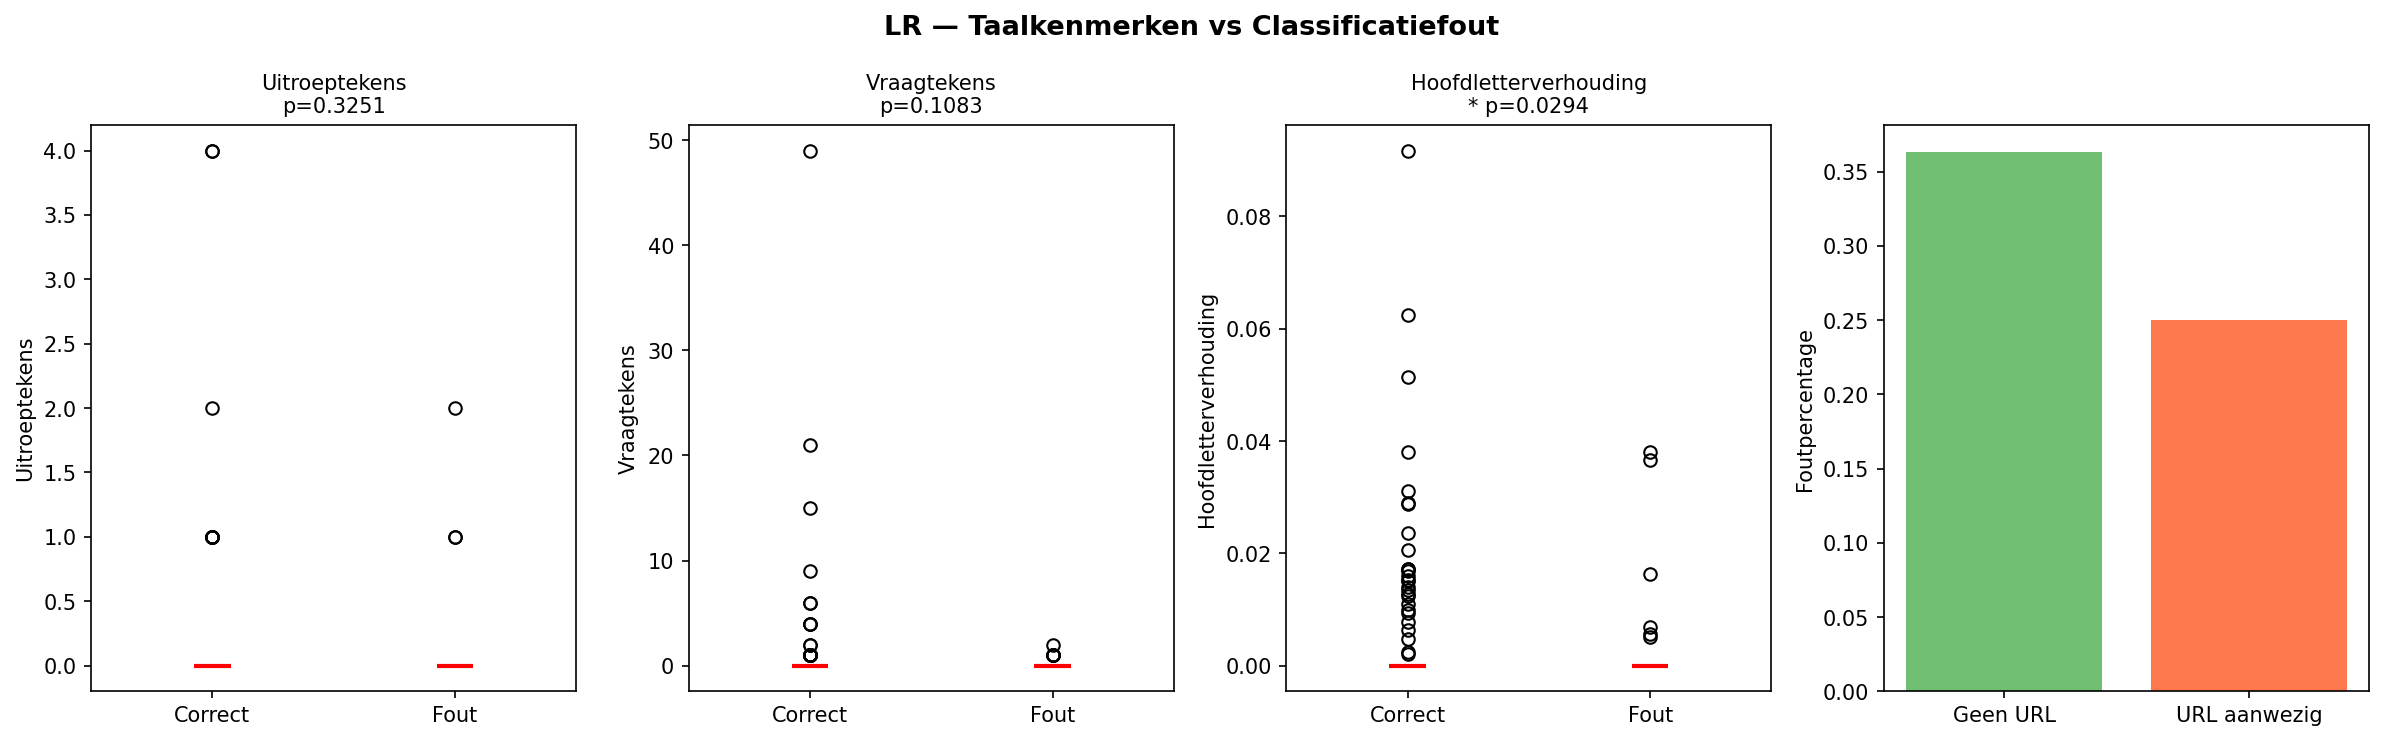
\includegraphics[width=0.75\textwidth]{../results/figures/taalgebruik_lr.png}
\caption{Top kenmerken voor Logistic Regression (waar/onwaar)}
\label{fig:lr_features}
\end{figure}

\section{SVM: Support Vector Machine}

\textbf{Bestand}: \texttt{src/models/train\_svm.py}

SVM is geselecteerd omdat het sterke theoretische garanties biedt voor
hoge-dimensionale, sparse feature-ruimtes zoals TF-IDF. Dit model is in de
literatuur een gebruikelijke keuze voor tekstclassificatie en vormt een goed
contrast met de lineaire LR-baseline en het semantische BERT-model.

\begin{lstlisting}[language=Python, basicstyle=\ttfamily\scriptsize,
  caption={SVM training pipeline with probabilistic calibration},
  literate={_}{\_}1]
from sklearn.svm import LinearSVC
from sklearn.calibration import CalibratedClassifierCV
from sklearn.pipeline import Pipeline
from sklearn.feature_extraction.text import TfidfVectorizer

pipeline = Pipeline([
    ('tfidf', TfidfVectorizer(
        max_features=50000, ngram_range=(1, 2),
        min_df=2, max_df=0.95, sublinear_tf=True
    )),
    ('svm', CalibratedClassifierCV(
        LinearSVC(C=1.0, class_weight='balanced', max_iter=10000)
    ))
])

pipeline.fit(X_train, y_train)
y_pred = pipeline.predict(X_test)
y_proba = pipeline.predict_proba(X_test)[:, 1]
\end{lstlisting}

De \texttt{Pipeline} combineert opnieuw TF-IDF met een classifier. \texttt{LinearSVC}
wordt gebruikt in plaats van de standaard \texttt{SVC} omdat het veel sneller is
voor grote, sparse datasets. \texttt{LinearSVC} werkt goed met de hoge-dimensionale
word-vectoren die uit TF-IDF voortkomen.

\texttt{CalibratedClassifierCV} wikkelt de SVM in een calibratiemodel. Een
klassieke SVM kan wel een klasse-label voorspellen (waar/onwaar), maar geeft
niet altijd betrouwbare kansschattingen. Door calibratie te gebruiken
kunnen we \texttt{predict\_proba} oproepen en AUC-ROC berekenen, wat belangrijk is
voor de evaluatie van mispredicties in plaats van alleen accuracy.

\texttt{class\_weight='balanced'} compenseert de ongelijke verdeling tussen de
labels en zorgt ervoor dat het model niet alleen focust op de meerderheidsklasse.

\section{BERT: Transformers}

\textbf{Bestand}: \texttt{src/models/train\_bert.py}

Model: \texttt{bert-base-uncased} (12 lagen, 768 hidden, 110M parameters)

\begin{lstlisting}[language=Python, basicstyle=\ttfamily\scriptsize,
  caption={BERT model fine-tuning script},
  literate={_}{\_}1]
from transformers import AutoTokenizer, AutoModelForSequenceClassification
from transformers import Trainer, TrainingArguments

tokenizer = AutoTokenizer.from_pretrained('bert-base-uncased')
model = AutoModelForSequenceClassification.from_pretrained(
    'bert-base-uncased', num_labels=2)

# Tokenisatie
def tokenize_function(examples):
    return tokenizer(examples['text'],
        padding='max_length', truncation=True, max_length=128)

train_dataset = train_dataset.map(tokenize_function, batched=True)
val_dataset = val_dataset.map(tokenize_function, batched=True)

# Training
training_args = TrainingArguments(
    output_dir='./results/bert/best_model',
    num_train_epochs=4,
    per_device_train_batch_size=16,
    learning_rate=2e-5,
    warmup_ratio=0.1,
    weight_decay=0.01,
    metric_for_best_model='f1',
    load_best_model_at_end=True,
    eval_strategy='steps',
    save_steps=100,
    eval_steps=100,
)

trainer = Trainer(model=model, args=training_args,
    train_dataset=train_dataset, eval_dataset=val_dataset)
trainer.train()
\end{lstlisting}

BERT is gekozen omdat het de volledige woordvolgorde en context van een bericht
kan modelleren. Mastodon-berichten kunnen subtiele semantische signalen en
contextuele nuance bevatten die niet goed door eenvoudige bag-of-words
representaties worden vastgelegd.

De tokenisatie stap zet de ruwe tekst om in tokens die door het voorgetrainde
BERT-model begrepen worden. \texttt{padding='max\_length'} en
\texttt{truncation=True} zorgen ervoor dat alle inputs dezelfde lengte krijgen,
waardoor batches efficiënt verwerkt kunnen worden.

De trainingsinstellingen zijn gekozen om BERT met een relatief lage
learning rate en een korte finetuning te trainen. \texttt{load\_best\_model\_at\_end=True}
zorgt ervoor dat het beste model op basis van de F1-score wordt bewaard.

\textbf{GPU-optimalisatie}: halveer de
\texttt{per\_device\_train\_batch\_size} of verhoog gradient accumulation
steps wanneer er onvoldoende VRAM beschikbaar is.

\section{Hyperparameter-tuning}

Voor SVM en Logistic Regression:

\begin{verbatim}
python src/models/train_svm.py --grid-search
python src/models/train_logistic_regression.py --grid-search
\end{verbatim}

Voor BERT: experimenteer met learning rate en batch size in config.yaml.

% ══════════════════════════════════════════════════════════════════
\section{Uitvoering van de pipeline}\label{sec:uitvoering}
% ══════════════════════════════════════════════════════════════════

\section{Installatie}

\begin{verbatim}
# 1. Kloon de repository
git clone <repository-url>
cd misinformatie_detectie

# 2. Maak een virtuele omgeving aan
python -m venv venv
venv\Scripts\activate          # Windows
# source venv/bin/activate     # Linux/Mac

# 3. Installeer afhankelijkheden
pip install -r requirements.txt
pip install -e .

# 4. Kopieer .env.example en vul je token in
copy .env.example .env
\end{verbatim}

\section{Volledige pipeline uitvoeren}

\begin{verbatim}
# Volledige pipeline (inclusief Mastodon-verzameling)
python run_pipeline.py

# Zonder Mastodon (gelabeld bestand al aanwezig)
python run_pipeline.py --skip-mastodon

# Zonder BERT (sneller, alleen SVM + LR)
python run_pipeline.py --skip-mastodon --skip-bert

# Met grid search voor hyperparameter-optimalisatie
python run_pipeline.py --skip-mastodon --grid-search

# Alleen evaluatie (modellen al getraind)
python run_pipeline.py --eval-only
\end{verbatim}

\section{Individuele stappen uitvoeren}

\begin{verbatim}
# Stap 1a: LIAR verwerken
python src/preprocessing/liar_preprocessor.py

# Stap 1b: Mastodon-berichten verzamelen
python src/preprocessing/mastodon_collector.py

# Stap 1c: Datasets samenvoegen
python src/preprocessing/data_merger.py

# Stap 2a: SVM trainen
python src/models/train_svm.py

# Stap 2b: Logistic Regression trainen
python src/models/train_logistic_regression.py

# Stap 2c: BERT fine-tunen
python src/models/train_bert.py

# Stap 3: Eindevaluatie
python src/evaluation/evaluate_all.py

# Stap 4: Factoranalyse
python src/evaluation/factor_analysis.py
\end{verbatim}

\section{Gegenereerde uitvoerbestanden}

Na een volledige pipeline-run zijn de volgende bestanden beschikbaar:

\begin{table}[H]
\centering
\caption{Gegenereerde bestanden na pipeline-uitvoering}
\begin{tabular}{ll}
\toprule
\textbf{Bestand} & \textbf{Inhoud} \\
\midrule
\texttt{results/model\_comparison\_test.csv} & F1/precision/recall per model \\
\texttt{results/svm/svm\_model.joblib} & Getraind SVM-model \\
\texttt{results/svm/svm\_top\_features.csv} & Top-50 discriminerende kenmerken \\
\texttt{results/lr/lr\_model.joblib} & Getraind LR-model \\
\texttt{results/lr/lr\_top\_waar\_features.csv} & Top kenmerken voor klasse ``waar'' \\
\texttt{results/bert/best\_model/} & Beste BERT-checkpoint \\
\texttt{results/bert/bert\_training\_history.csv} & Verlies/F1 per epoch \\
\texttt{results/factor\_taalgebruik\_statistieken.csv} & Mann-Whitney U resultaten \\
\texttt{results/figures/*.png} & Alle grafieken en visualisaties \\
\bottomrule
\end{tabular}
\end{table}

\section{Reproduceerbaarheid en versiebeheer}
\label{sec:reproduceerbaarheid}
% ══════════════════════════════════════════════════════════════════

\subsection{Random seed}

Alle willekeurige processen (datasplitsing, modelinitialisatie, dataschudding)
gebruiken een vaste seed van \textbf{42}, ingesteld via de functie
\texttt{set\_seed()} in \texttt{src/utils.py}. Dit garandeert dat resultaten
volledig reproduceerbaar zijn.

\subsection{Git-versiebeheer}

De repository bevat een \texttt{.gitignore} die voorkomt dat gevoelige
bestanden (API-tokens in \texttt{.env}) of grote bestanden
(modelgewichten, ruwe dataset) worden gecommit.

Aanbevolen commitstrategie:

\begin{verbatim}
git add src/ notebooks/ config.yaml requirements.txt
git commit -m "feat: SVM baseline getraind (val F1=0.XX)"
\end{verbatim}

\subsection{Configuratiebeheer}

Alle hyperparameters en paden zijn gecentraliseerd in \texttt{config.yaml}.
Dit betekent dat experimenten kunnen worden herhaald of aangepast zonder
de broncode te wijzigen.

% ══════════════════════════════════════════════════════════════════
\chapter{Evaluatie en analyse}\label{ch:evaluatie}

\section{Evaluatiemetrieken}

Alle modellen worden beoordeeld op een onafhankelijke testset. Gebruikte
metrieken (berekend in \texttt{src/evaluation/metrics.py}):

\begin{table}[H]
\centering
\caption{Evaluatiemetrieken}
\begin{tabular}{ll}
\toprule
\textbf{Metriek} & \textbf{Beschrijving} \\
\midrule
Accuracy & \% correct geclassificeerde berichten \\
F1 (macro) & Harmonisch gemiddelde per klasse (aangewezen bij onbalans) \\
F1 (binary) & F1 voor klasse ``waar'' alleen \\
Precision & Van voorspelde ``waar'': \% echt waar \\
Recall & Van werkelijke ``waar'': \% correct geïdentificeerd \\
AUC-ROC & Discriminerend vermogen \\
\bottomrule
\end{tabular}
\end{table}

\section{Modelevaluatie}

Via \texttt{src/evaluation/evaluate\_all.py} worden gegenereerd:

\begin{verbatim}
python src/evaluation/evaluate_all.py
\end{verbatim}

\subsection{Metriekvergelijking}

\begin{figure}[H]
\centering
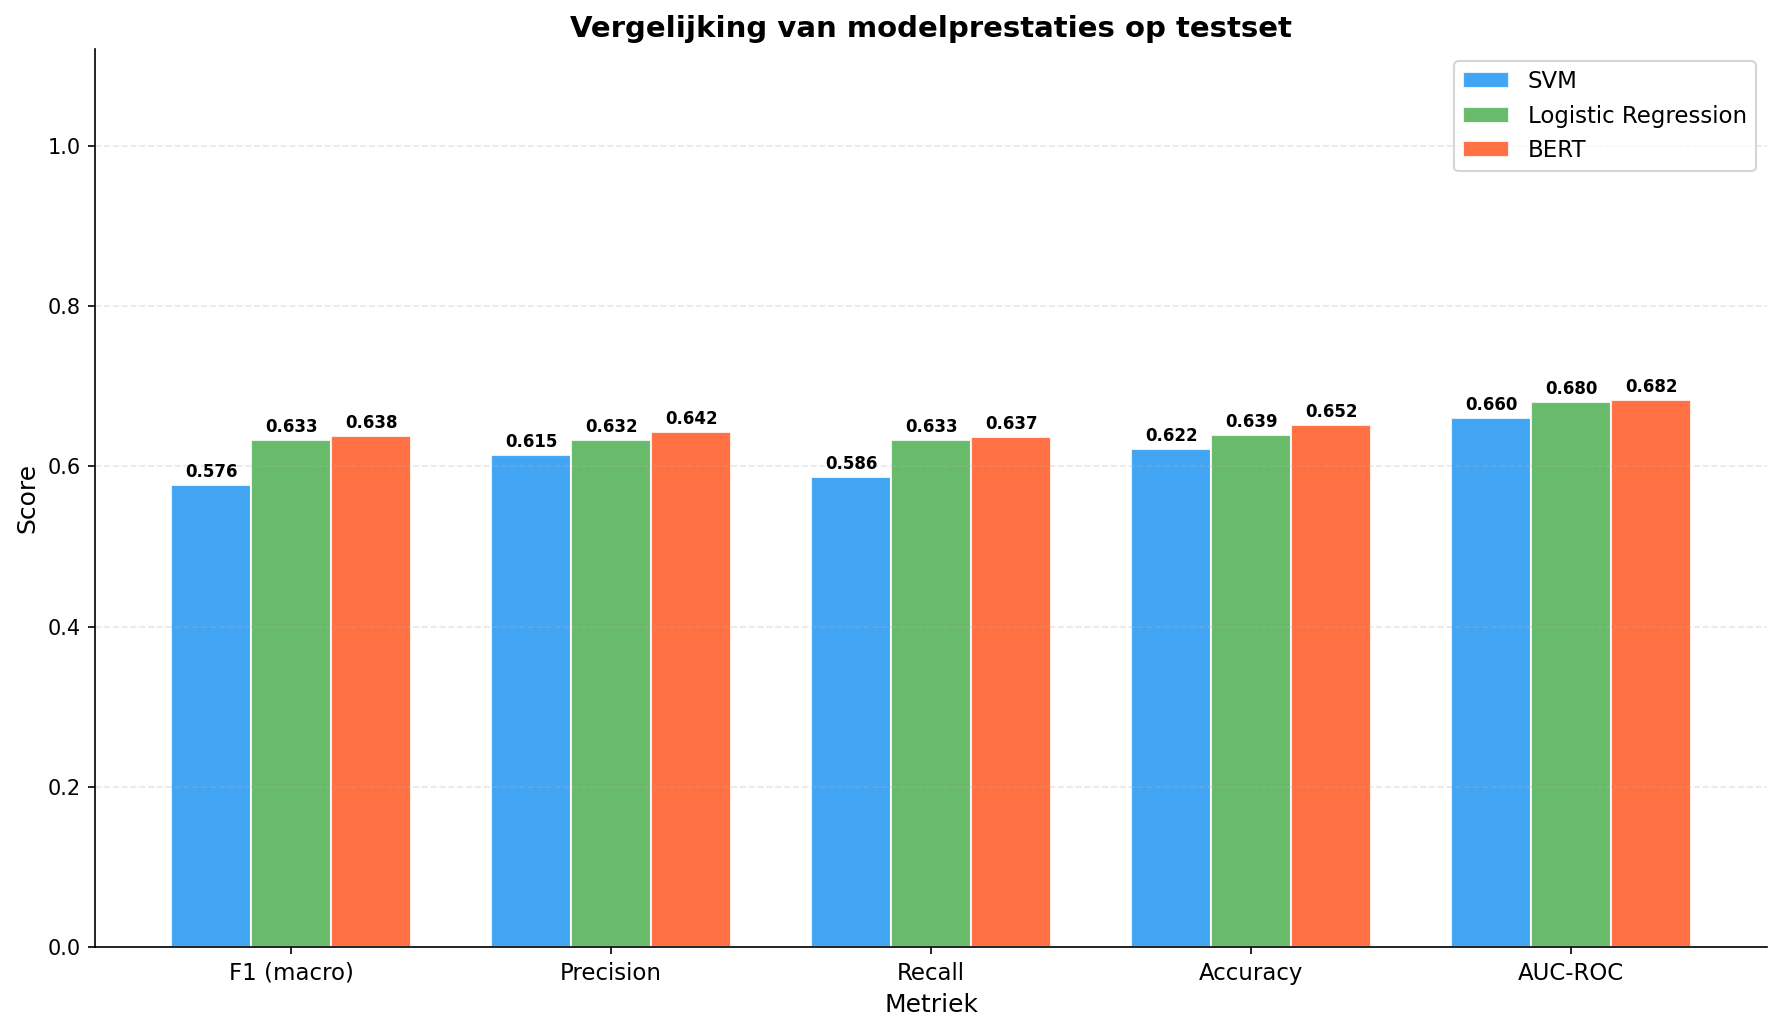
\includegraphics[width=0.8\textwidth]{../results/figures/metrics_comparison.png}
\caption{Vergelijking van F1, Precision, Recall en Accuracy per model (SVM, LR, BERT)}
\label{fig:metrics}
\end{figure}

\subsection{Verwarringsmatrices}

\begin{figure}[H]
\centering
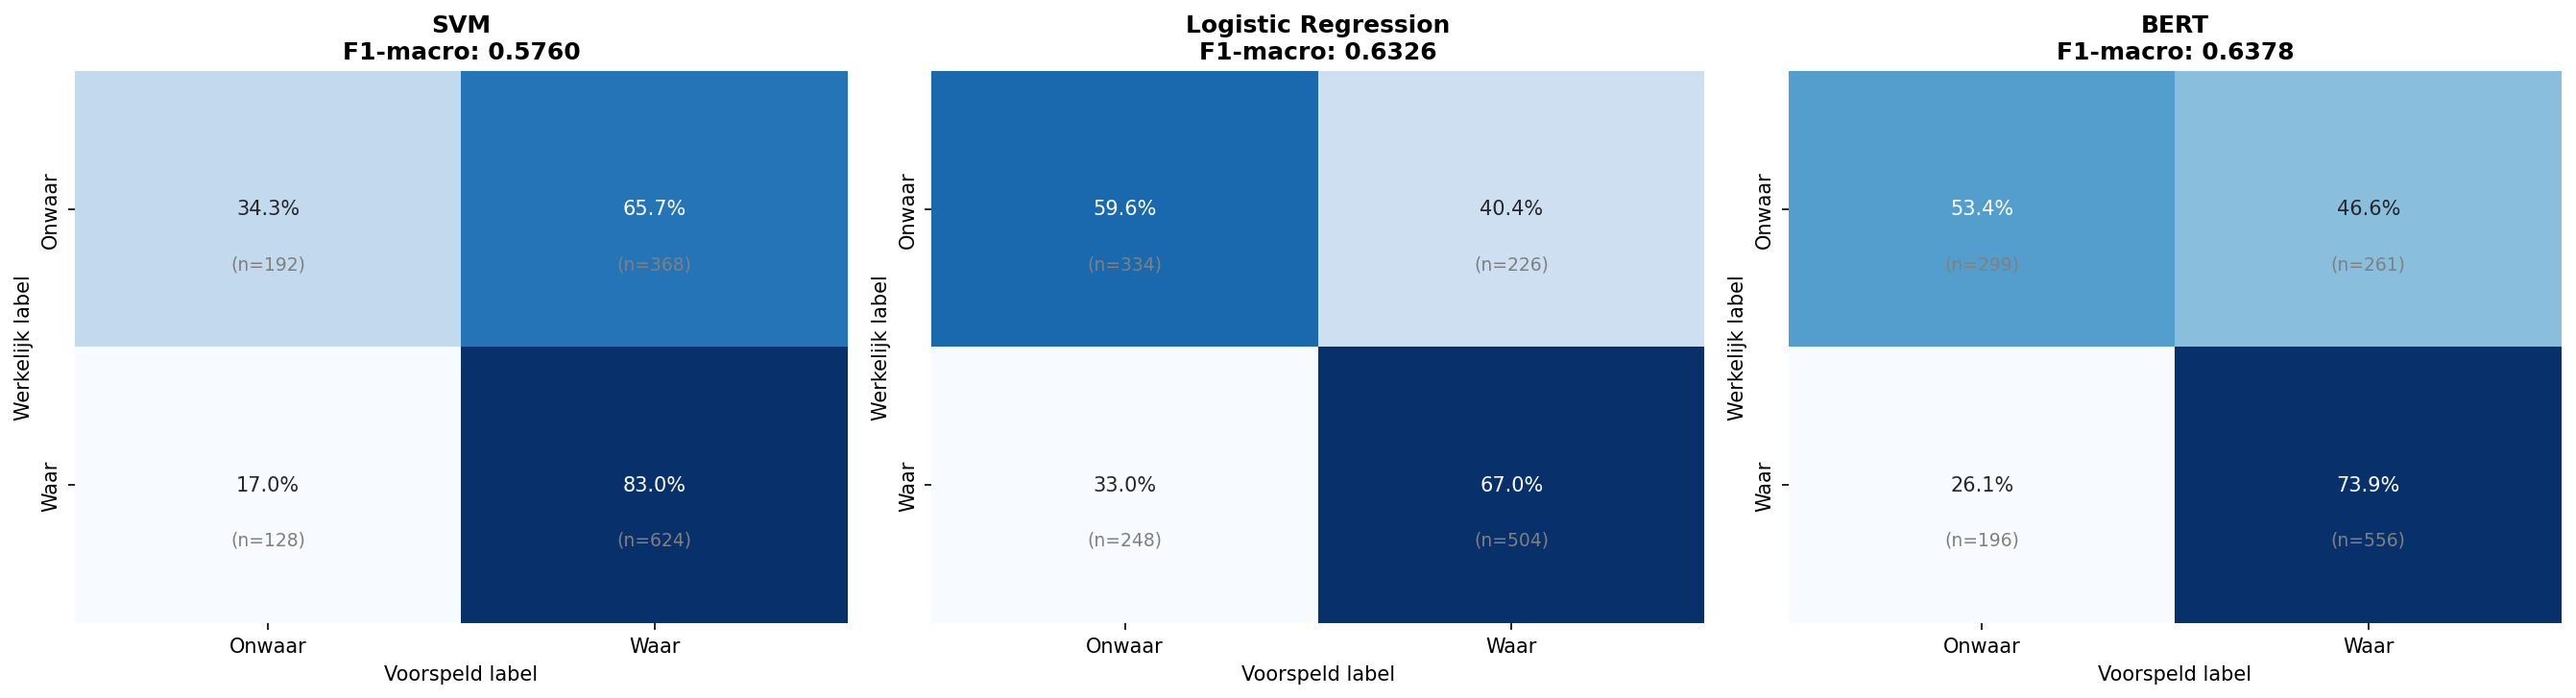
\includegraphics[width=0.85\textwidth]{../results/figures/confusion_matrices.png}
\caption{Verwarringsmatrices voor alle drie modellen op testset. Opmerking: metrieke labels in figuur verwijzen naar F1-macro (niet F2-macro).}
\label{fig:confusion}
\end{figure}

\subsection{ROC-curves}

\begin{figure}[H]
\centering
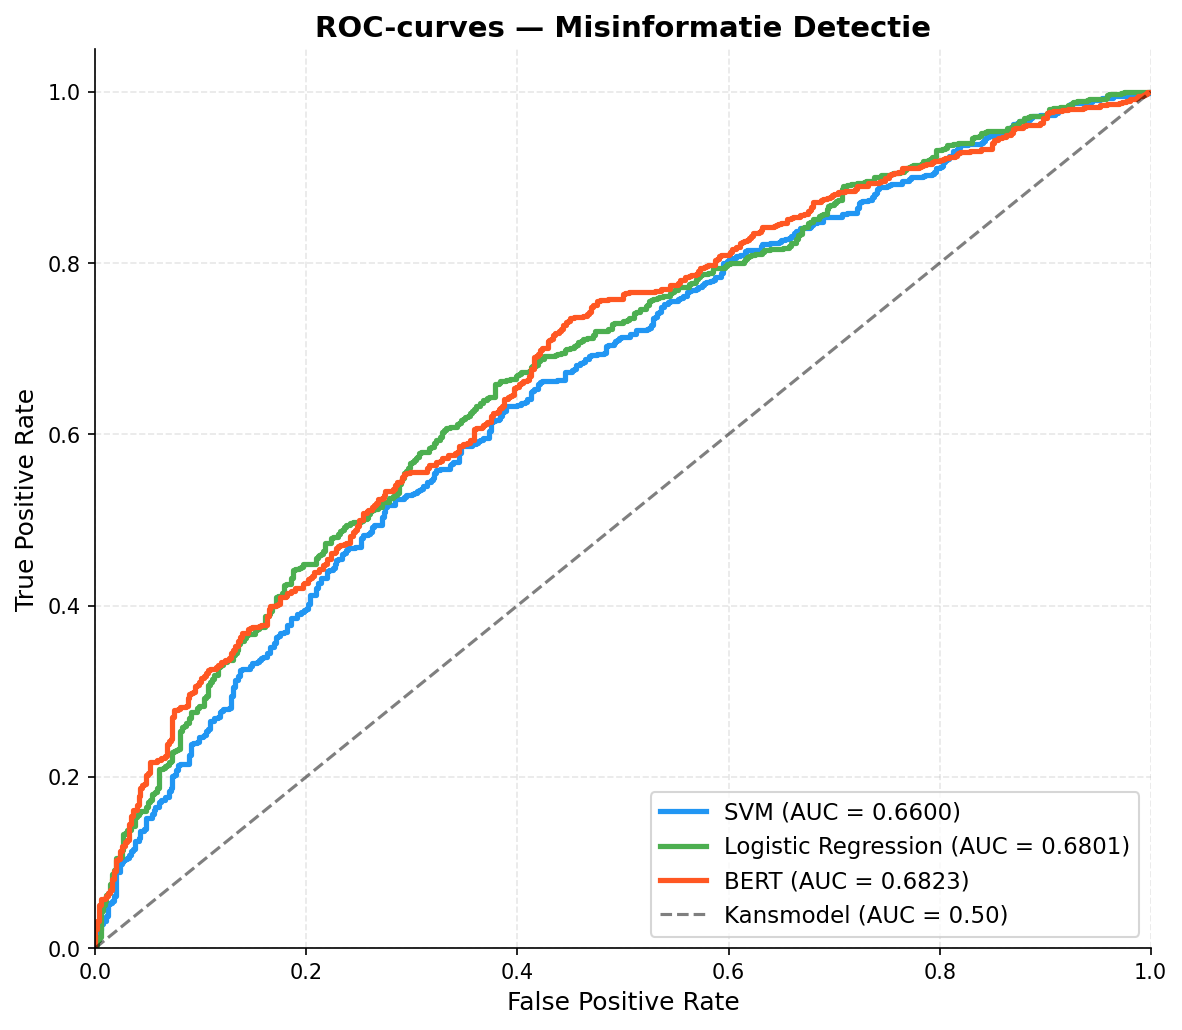
\includegraphics[width=0.75\textwidth]{../results/figures/roc_curves.png}
\caption{ROC-curves met AUC-scores per model}
\label{fig:roc}
\end{figure}

\begin{figure}[H]
\centering
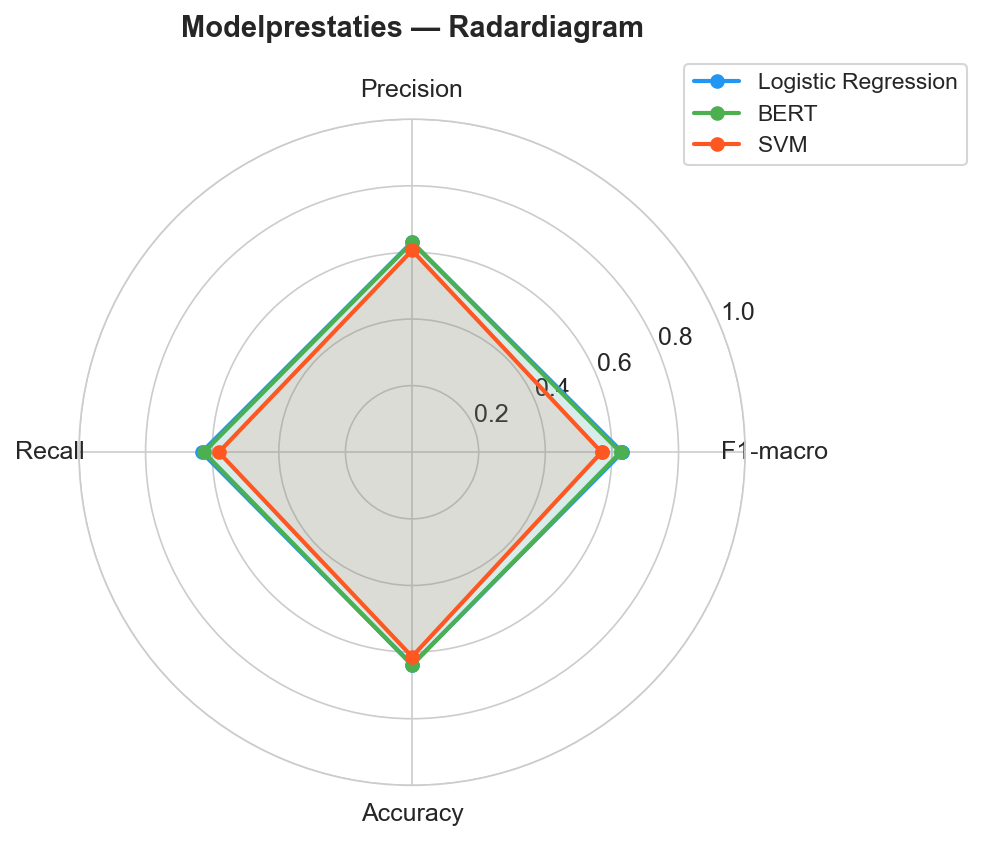
\includegraphics[width=0.7\textwidth]{../results/figures/radar_vergelijking.png}
\caption{Radardiagram van modelprestaties}
\label{fig:radar}
\end{figure}

\section{Factoranalyse}

Via \texttt{src/evaluation/factor\_analysis.py} worden:

\begin{verbatim}
python src/evaluation/factor_analysis.py
\end{verbatim}

\subsection{Factor 1: Berichtlengte}

Chi-square test (per lengtecategorie). Resultaten in \texttt{factor\_length\_analysis.csv}.

\begin{figure}[H]
\centering
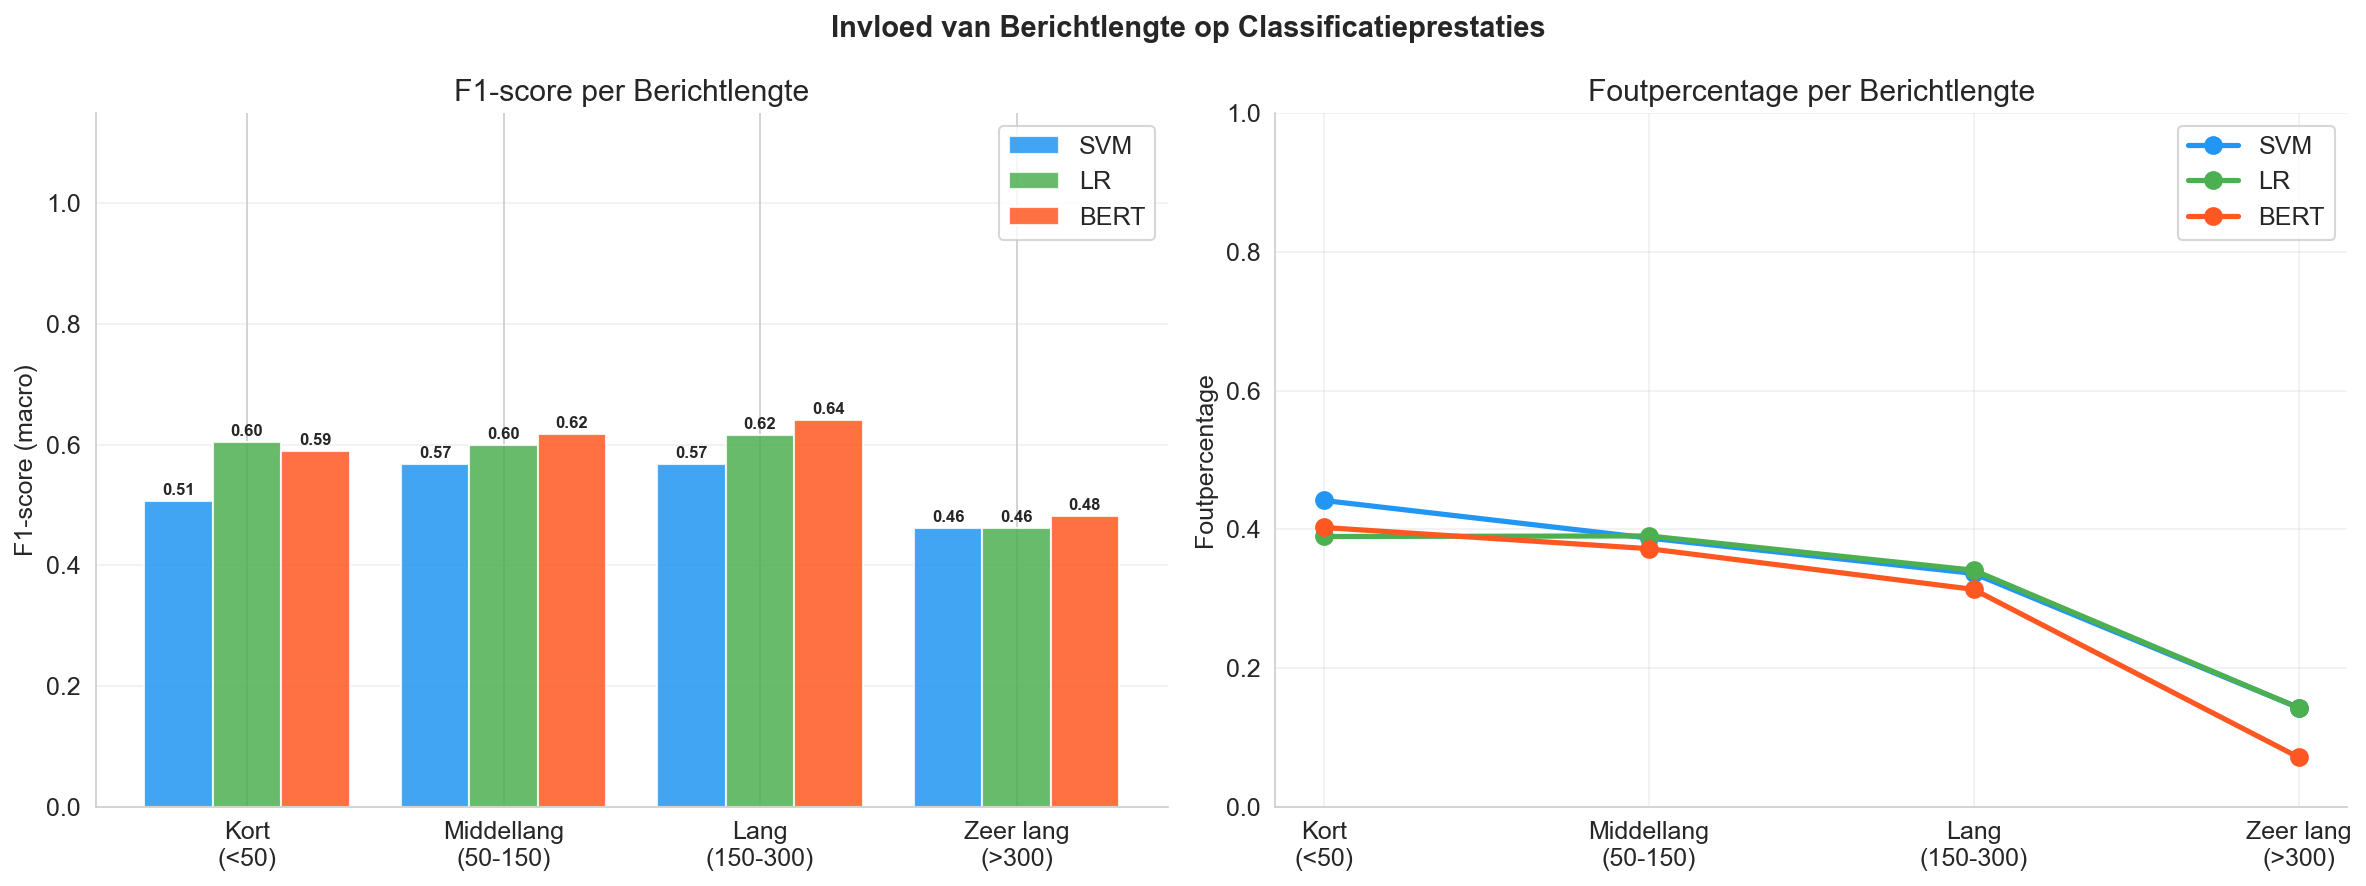
\includegraphics[width=0.75\textwidth]{../results/figures/analyse_berichtlengte.png}
\caption{Invloed van berichtlengte op classificatiefout per model}
\label{fig:length}
\end{figure}

\subsection{Factor 2: Bronbetrouwbaarheid}

ANOVA (laag/middel/hoog). Resultaten in \texttt{factor\_trust\_analysis.csv}.

\begin{figure}[H]
\centering
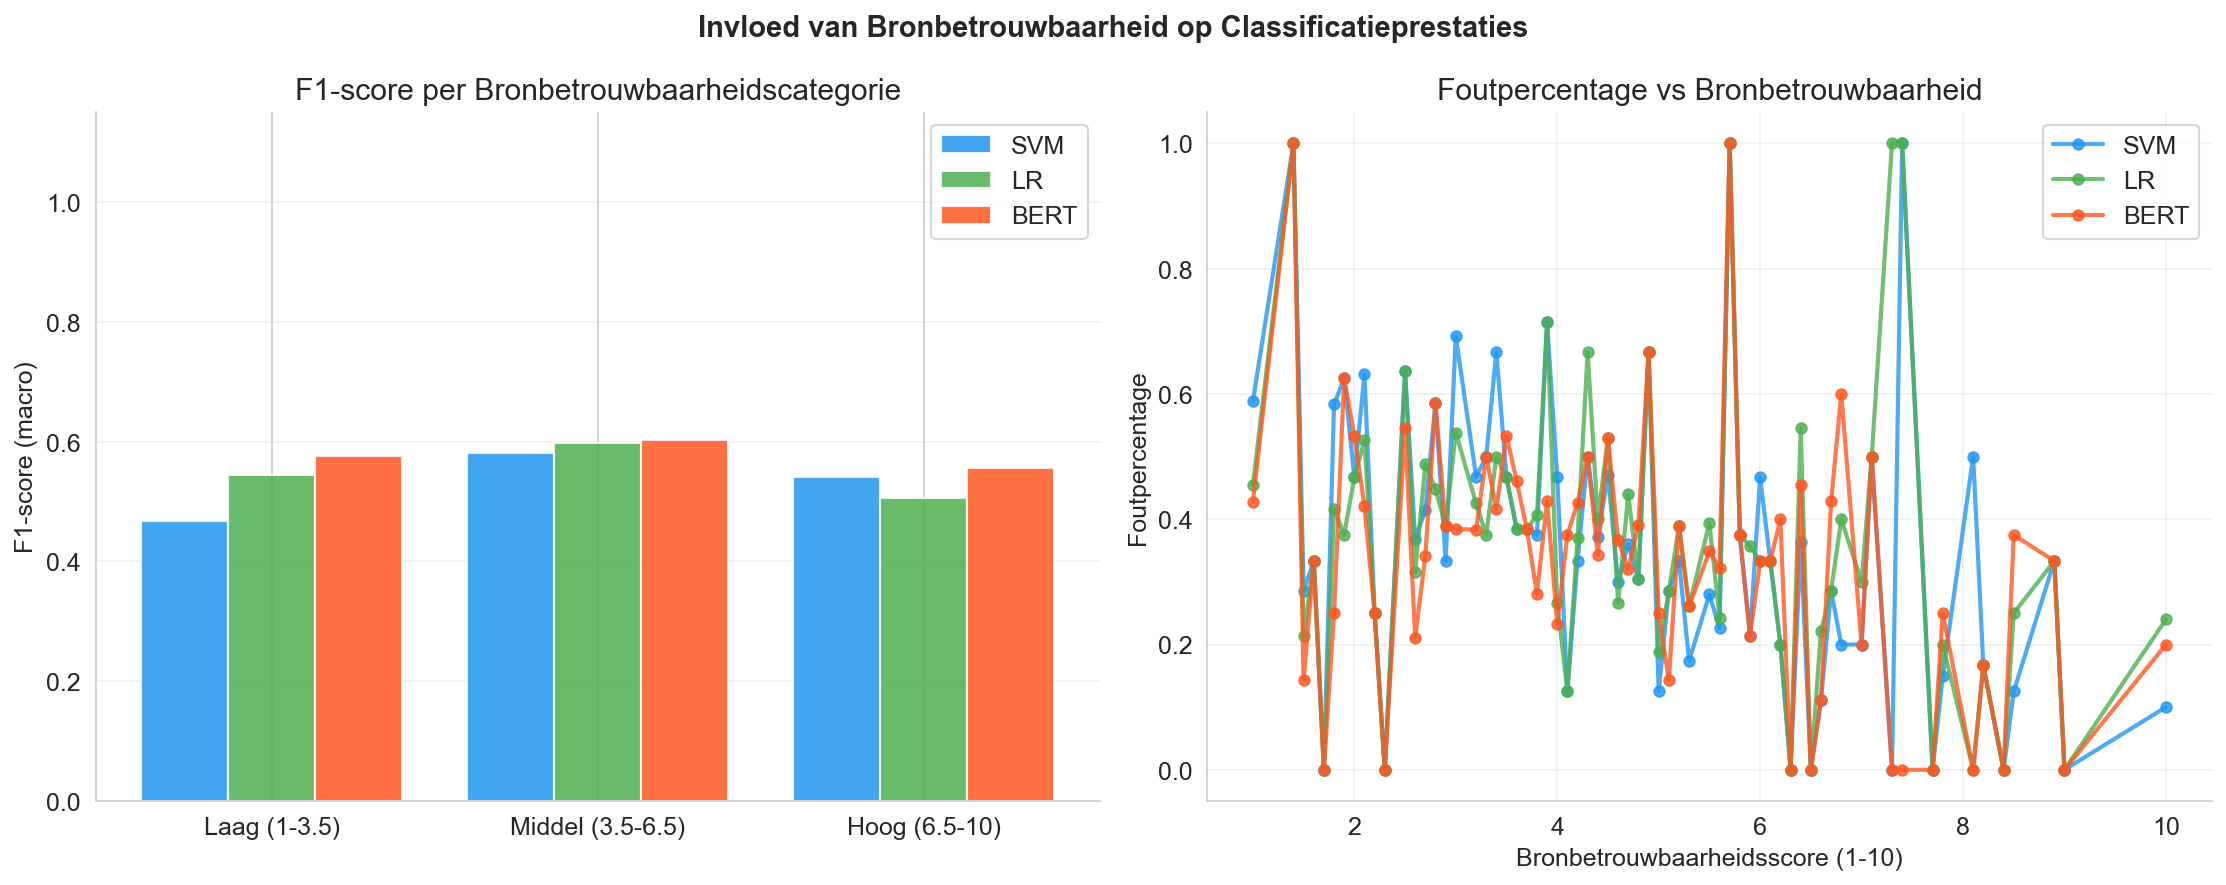
\includegraphics[width=0.75\textwidth]{../results/figures/analyse_bronbetrouwbaarheid.png}
\caption{Invloed van bronbetrouwbaarheid op modelprestaties}
\label{fig:trust}
\end{figure}

\subsection{Factor 3: Taalgebruik}

Mann-Whitney U toets voor exclamatie's, vragen, CAPS, URLs.
Resultaten in \path{factor_taalgebruik_statistieken.csv}.

\begin{figure}[H]
\centering
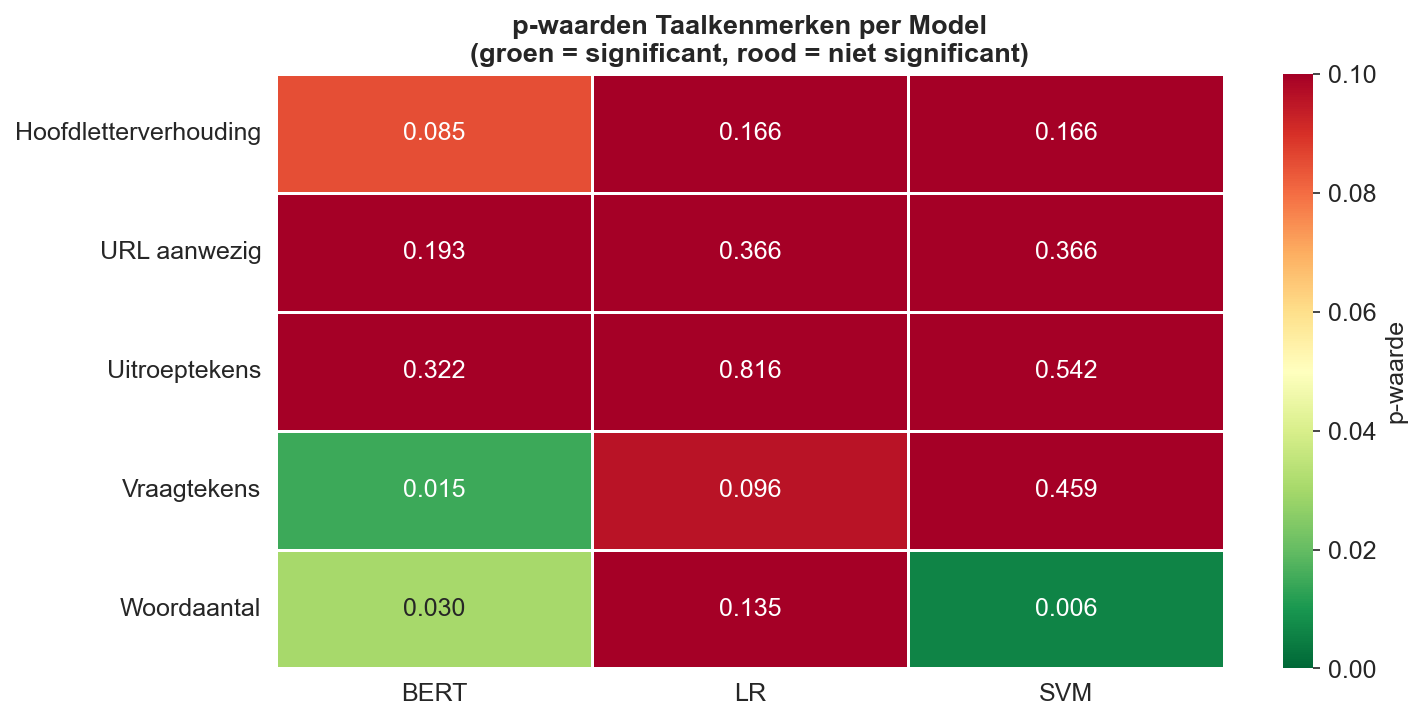
\includegraphics[width=0.8\textwidth]{../results/figures/heatmap_taalkenmerken.png}
\caption{Heatmap van p-waarden voor taalgebruikskenmerken (SVM en LR)}
\label{fig:linguistic}
\end{figure}

\section{Analyse Jupyter Notebook}

Volledige visualisatie in \texttt{notebooks/02\_analyse\_rapport.ipynb}.
Enkele belangrijke figuren:

\subsection{BERT trainingsverloop}

\begin{figure}[H]
\centering
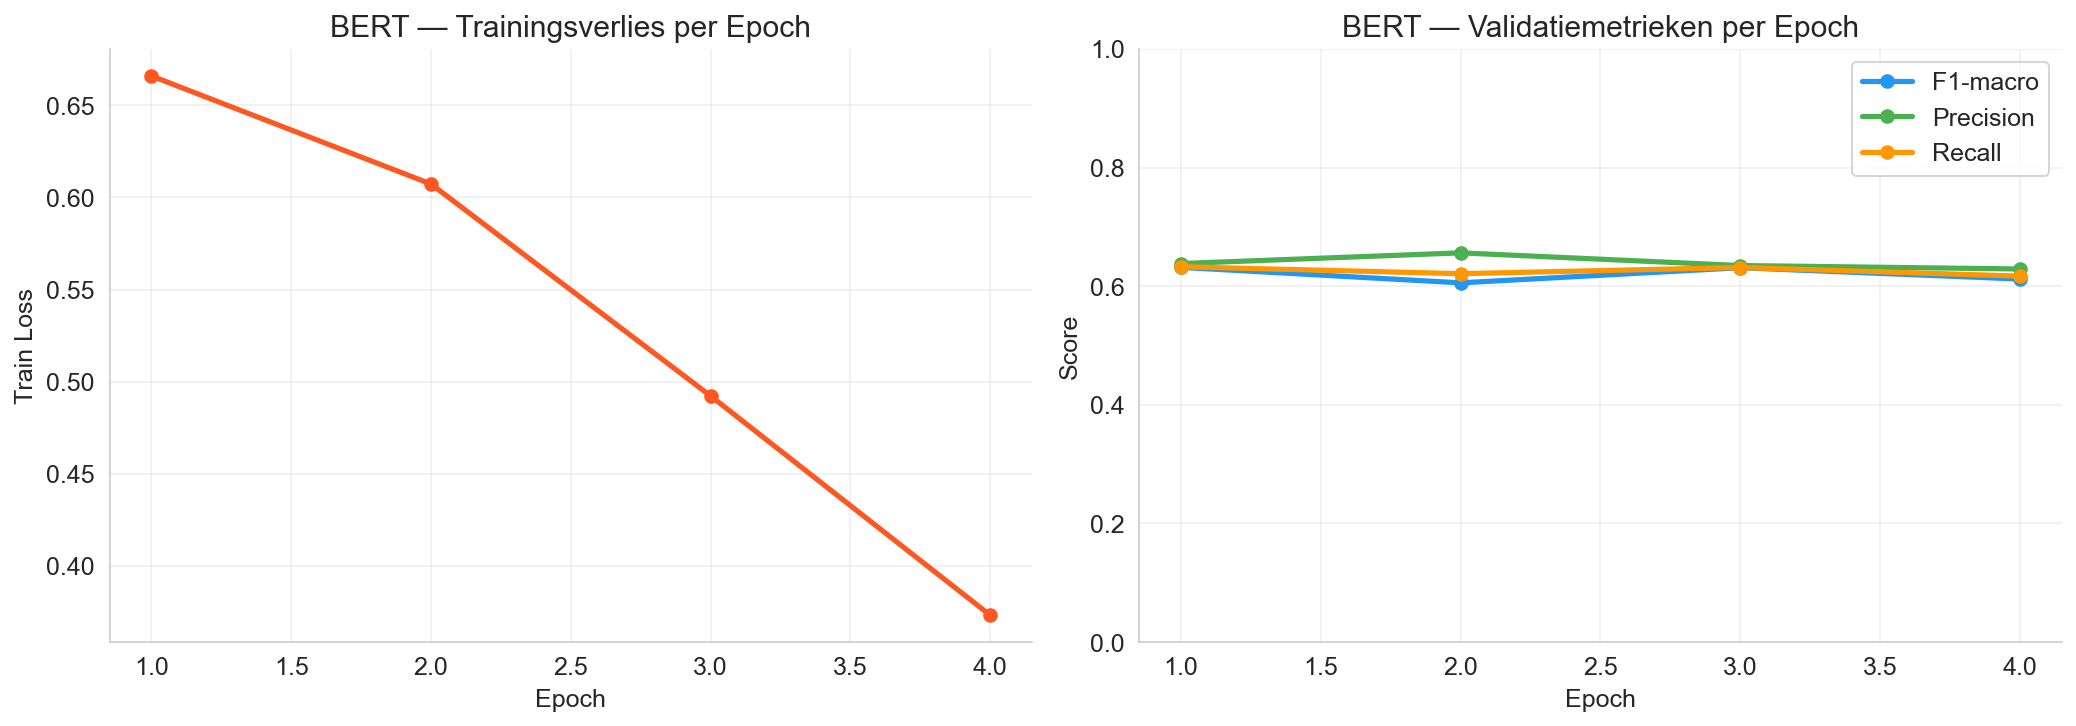
\includegraphics[width=0.75\textwidth]{../results/figures/bert_trainingsverloop.png}
\caption{Trainings- en validatieverlies + F1-macro per epoch}
\label{fig:bert}
\end{figure}

\subsection{F1-score per berichtlengte}

\begin{figure}[H]
\centering
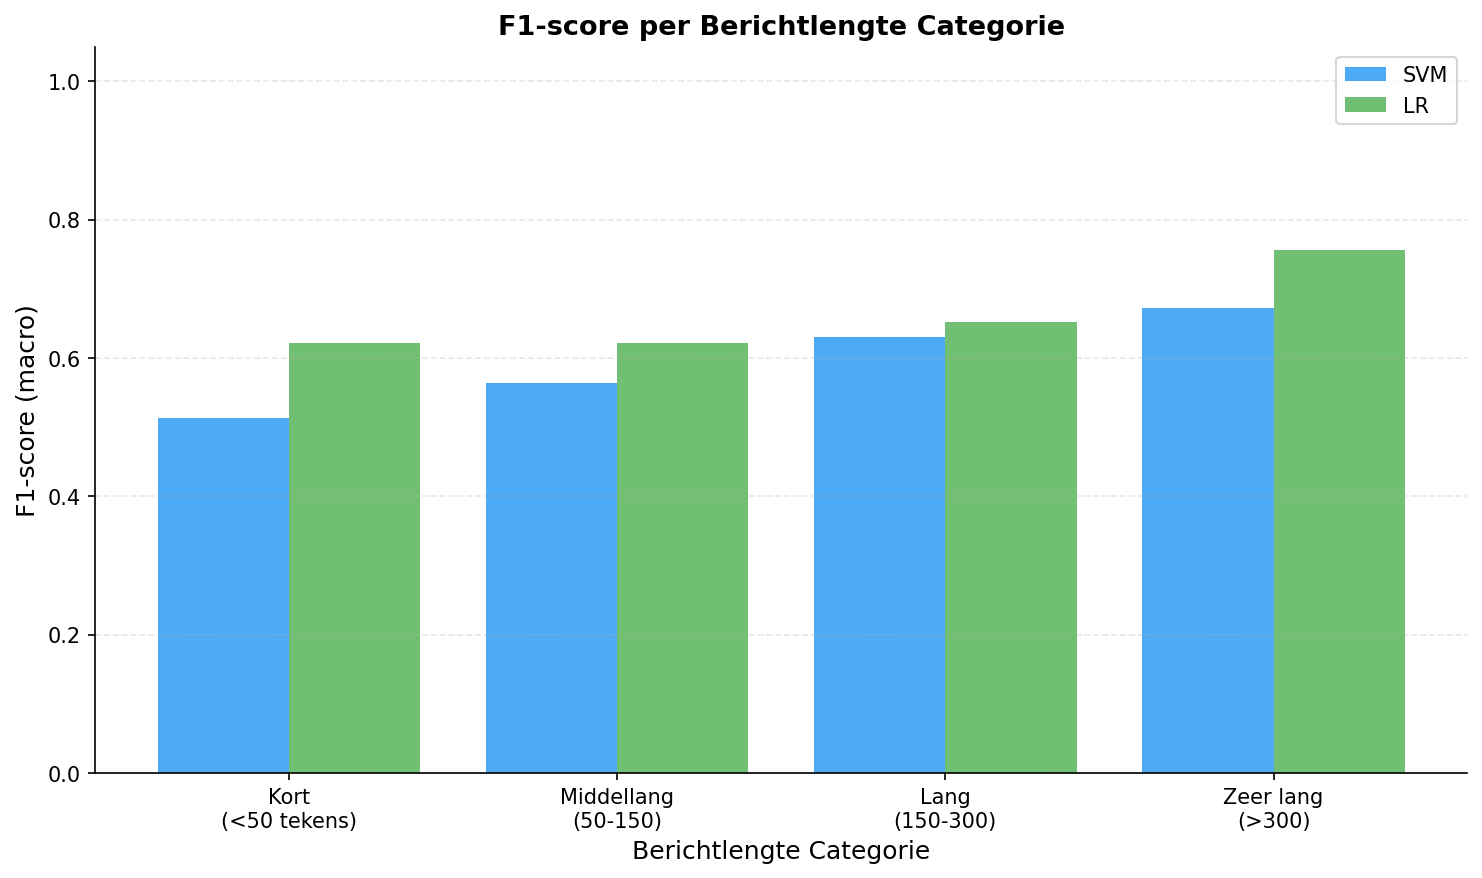
\includegraphics[width=0.75\textwidth]{../results/figures/f1_per_lengte.png}
\caption{Modelprestaties uitgesplitst naar berichtlengte}
\label{fig:f1length}
\end{figure}

\subsection{Exploratieve data-analyse}

Zie ook \texttt{notebooks/01\_eda.ipynb} voor labelbalans, wordclouds en correlatiematrices:

\begin{figure}[H]
\centering
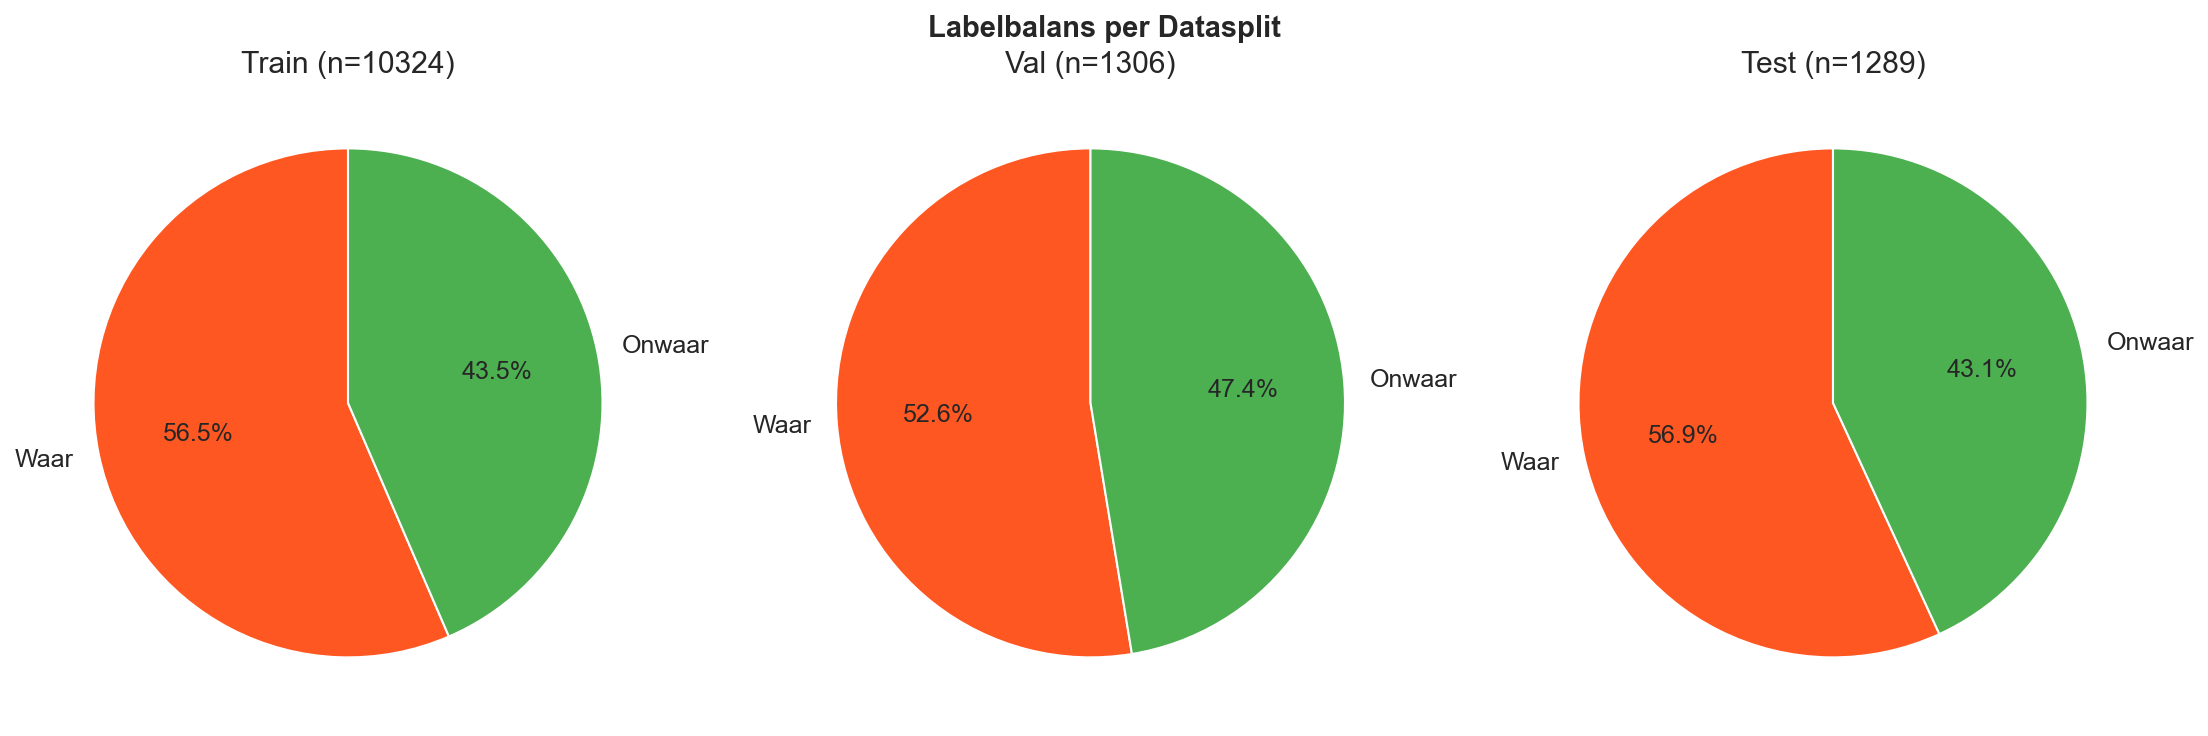
\includegraphics[width=0.75\textwidth]{../results/figures/eda_labelbalans.png}
\caption{Balans van waar/onwaar berichten in dataset}
\label{fig:balance}
\end{figure}

